\documentclass{beamer}

\usepackage[utf8]{inputenc}
\usepackage[T1]{fontenc}
\usepackage{lmodern}
\usepackage[australian]{babel}

\usepackage[style=verbose,citestyle=authortitle-comp]{biblatex}
\addbibresource{slides.bib}
\usepackage{xpatch}
\xapptobibmacro{cite}{\setunit{\nametitledelim}\printfield{year}}{}{}
\AtBeginBibliography{\footnotesize}
\let\oldfootnotesize\footnotesize
\renewcommand*{\footnotesize}{\oldfootnotesize\tiny}

\usepackage{csquotes}

\usepackage{amsthm,amsfonts,amssymb,amsmath,mathtools,graphicx}

\usepackage{wasysym}

\usetheme{metropolis}

\renewcommand{\leq}{\leqslant}
\renewcommand{\geq}{\geqslant}

\usepackage{ragged2e}
\usepackage{etoolbox}
\apptocmd{\frame}{}{\justifying}{}

\usepackage{relsize}
\newcommand\CC{C\nolinebreak[4]\hspace{-.05em}\raisebox{.4ex}{\relsize{-3}{\textbf{++}}}}

\usefonttheme[onlymath]{serif}

\author{Alex Bishop}
\title{Group Geodesic Growth}
%\subtitle{}
%\logo{}
\institute{University of Technology, Sydney}
\date{29 June 2018}
%\subject{}
%\setbeamercovered{transparent}
%\setbeamertemplate{navigation symbols}{}

\usepackage{tikz}

\newcommand{\aActionNotation}{{\tikz{\fill[black]  (-1,-1) -- (-1.1,-1.25) -- (-0.9,-1.25) -- cycle;}}}
\newcommand{\eActionNotation}{{\tikz{\draw (0,-1) -- (-1.1+1,-1.25) -- (-0.9+1,-1.25) -- cycle;}}}

\begin{document}

\begin{frame}[plain]
	\maketitle
\end{frame}

\section{Notation}

\begin{frame}{Volume Growth}
Given a group, $G$, with some finite symmetric generating set, $X = X^{-1}$, we can define the length of any element $g \in G$ as the length of the shortest word $w \in X^\star$ equivalent to $g$.
\[
  \left\Vert g \right\Vert_X
  \coloneqq
  \min
  \left\{
    n \in \mathbb{N}
    \, \middle\vert \,
    x_1 x_2 \cdots x_n =_G g \text{ with each } x_j \in X
  \right\}
\]
Then, $G$ becomes a homogeneous geodesic metric space with metric
\[
  d_X(g,h) \coloneqq \left\Vert g h^{-1} \right\Vert_X
\]
Then, the (volume) growth function $f_X(n)$ will be the volume of a closed ball of radius $n$.
That is,
\[
  f_X(n) \coloneqq \#\left\vert
  	\left\{
  	  g \in G
  	  \,:\,
  	  \left\Vert g \right\Vert_X \leq n
  	\right\}
   \right\vert
\]
Similarly, spherical growth will be defined as
\[
  s_X(n) \coloneqq \#\left\vert
  \left\{
  	g \in G
  \,:\,
  	\left\Vert g \right\Vert_X = n
  \right\}
  \right\vert
\]
\end{frame}

\begin{frame}{Usual Growth Relation}
Then, defining a partial order on such growth functions as
\[
  f \preccurlyeq g
  \iff
  \text{there exists a }C\in \mathbb{N}_+\text{ s.t. }
  f(n) \leq C \cdot g(C\cdot n)
\]
It is a classic result by \v{S}varc\footcite{SvarcEquivClass} and Milnor\footcite{MilnorEquivClass} that the corresponding equivalence relation
\[
  f\sim g \iff f \preccurlyeq g \text{ and } g \preccurlyeq f
\]
is invariant under quasi-isometry.
In particular, for any two symmetric generating sets $X$ and $Y$ of $G$ it is true that $f_X \sim f_Y$.
\end{frame}

\begin{frame}{Growth Types}
Then, the growth function, $f$, of a group is called:

\begin{tabular}{c r l}
\quad&\textbf{Polynomial:}&
If there exists an $d \in \mathbb{R}$ such that $f \preccurlyeq n^d$
\\
&&\textit{(the smallest such $d$ is called the degree)}
\\[0.5em]
\quad&\textbf{Exponential:}&
If it is true that $e^n \preccurlyeq f$
\\[0.5em]
\quad&\textbf{Intermediate:}&
If it is neither polynomial nor exponential
\end{tabular}

\vspace{0.5cm}

\visible<2>{
In 1968, Milnor asked the following question\footcite{Milnor1968}

\begin{quotation}
	Are all group growth functions either polynomial of integer degree or exponential?
\end{quotation}
}

\end{frame}



\begin{frame}{Milnor's Questions}
Milnor asked the following question\footcite{Milnor1968}

\begin{quotation}
	Are all group growth functions either polynomial of integer degree or exponential?
\end{quotation}

\vspace{0.25cm}

\visible<2->{
The first is a corollary to Gromov theorem\footcite{GromovTheorem} and that the all virtually nilpotent groups have growth of integer degree\footcite{PolynomialDegree}.
}

\vspace{0.25cm}

\visible<3->{
The second half was resolved by Grigorchuk when he showed a particular example to have intermediate growth\footcite{GrigInterm}.
}

\end{frame}



\section{Geodesic Growth}

\begin{frame}{Definition}
Given a finite symmetric generating set, $X$, the geodesic growth function, $F_X(n)$, will count the number of geodesics words within a ball of size $n$ starting from its centre. That is,
\[
	F_X(n)
	\coloneqq
	\#
	\left\vert
	\left\{
		x_1 x_2 \cdots x_k \in X^\star
		\, : \,
		\left\Vert x_1 x_2 \cdots x_k \right\Vert_X
		=
		k \leq n
	\right\}
	\right\vert
\]
\visible<2->{What's different?}
\visible<3->{
\begin{center}
No longer invariant under change of generating set!!!
\end{center}
}

\end{frame}


%\section{Open Questions}

%\begin{frame}
%\begin{itemize}
%	\item same as Milnor's original question except of geodesic growth
%	\begin{itemize}
%		\item intermediate growth
%		\item possible polynomial growths
%	\end{itemize}
%
%	\item how can we make this equivalence class ``make sense''
%	\begin{itemize}
%		\item it is not known if taking the $\liminf$ of growth will make sense
%	\end{itemize}
%
%	\item mention Julie's thesis \& Murray's idea
%	\begin{itemize}
%		\item eliminate Grigorchuk's group and many other w.r.t.\@ their usual generating set
%		\item polynomial Schreier graph for Fabrykowski-Gupta
%	\end{itemize}
%\end{itemize}
%\end{frame}

\begin{frame}{Questions}

\textbf{Question:}
What forms of polynomial geodesic growth are possible?

\vspace{0.5cm}

\visible<2->{
\textbf{Question:}
In what cases does it make sense to take the infimum of geodesic growth with respect to the equivalence relation on growth functions?
More generally, is there a way in which we define geodesic growth as an invariant of a group.
}

\vspace{0.5cm}

\visible<3->{
\textbf{Question:}
Does there exist a group with a generating set such that the geodesic growth function is intermediate?
What class of usual growth do they possess?
}

\end{frame}

%\begin{frame}
%\textbf{Polynomial Geodesic Growth:} (Bridson, Burillo, Elder and \v{S}uni\'c\footcite{OnGroupsPolynomial})
%
%\begin{theorem}[Theorem 1]
%	content...
%\end{theorem}
%
%\begin{theorem}[Theorem 2]
%	content...
%\end{theorem}
%
%\end{frame}

\begin{frame}{Main Question of Focus}
\textbf{Question:}
Does there exist a group with a generating set such that the geodesic growth function is intermediate?

\vspace{0.5em}

\textbf{Natural starting point:} Grigorchuk's group with usual generators

\visible<2->{
\qquad NO! -- has a sub-family of exponential geodesic growth
\\
{\hfill \small(Elder, Gutierrez, \v{S}uni\'c)}
}

\visible<3->{
\textbf{In fact:}\footcite{Julie2016GeodesicGrowth} (w.r.t.\@ usual generating sets)

\begin{tabular}{c r l}
	&Grigorchuk $G_\omega$:&
	\visible<4->{No}
	\\
	&Gupta-Sidki $p$-groups\footnote{not proven to be intermediate growth}:&
	\visible<5->{No}
	\\
	&Square group:&
	\visible<6->{No}
	\\
	&Spinal group:&
	\visible<7->{No}
	\\
	&Gupta-Fabrykowski: &
	\visible<8->{\dots}\visible<9->{\textit{maybe}}
	\\\ 
\end{tabular}
}

\end{frame}


\section{Fabrykowski-Gupta Group}

\begin{frame}{Regular Rooted Tree}
Each of its elements is an automorphism on a $3$-regular rooted tree
\begin{figure}
\centering
\includegraphics{figure/FabGup/regularTree}
\end{figure}
\end{frame}

\begin{frame}{Generators of Fabrykowski-Gupta}
In particular, the group is generated by actions $a$ and $b$ where
\begin{figure}
	\centering
	\hfill
	\begin{minipage}{0.45\linewidth}
		\centering
		\includegraphics[width=0.8\linewidth]{figure/FabGup/tAction}
	\end{minipage}
	\hfill
	\begin{minipage}{0.45\linewidth}
		\centering
		\includegraphics[width=0.8\linewidth]{figure/FabGup/zAction}
	\end{minipage}
	\hfill
	
	\vspace{1em}
	
	\hfill
	\begin{minipage}{0.45\linewidth}
		\centering
		Action of $a$
	\end{minipage}
	\hfill
	\begin{minipage}{0.45\linewidth}
		\centering
		Action of $b$
	\end{minipage}
	\hfill
\end{figure}
where \aActionNotation\ is an action by $a$ and \eActionNotation\ is the trivial action

\end{frame}

\section{Previous}

\begin{frame}{Experimental Computation}

In Honours\footnote{similar to a masters that's half corsework, half research} Thesis:
Attempted to explicitly compute the geodesics of the Fabrykoswki-Gupta group in the hopes of finding an exponential growth sub-family or some `obvious' pattern help realise intermediate geodesic growth

\visible<2->{
How:
\begin{itemize}
	\item[(1)] By defining an efficiently computable comparison on group elements an improved complexity over brute-forces
\visible<3->{\only<1-3>{
	\[
	\text{brute-force}
	\sim
	O\left(
	\sum_{\ell=1}^{n} s(\ell-1)^2 \  \ell \log \ell 
	\right)
	\]
}}
\only<4->{
	\[
	 O\left(
	 \sum_{\ell=1}^{n} s(\ell-1) \left( \log s(\ell-1) \right)^2
	 \ \ell \log \ell 
	 \right)
	\]
}
	
	\item<5-> [(2)]
	Implementing in C (later in \CC{11}) with multithreading
	\\\ 
\end{itemize}
}

\end{frame}

\begin{frame}{Experimental Computation}

In Honours Thesis:
Attempted to explicitly compute the geodesics of the Fabrykoswki-Gupta group in the hopes of finding an exponential growth sub-family or some `obvious' pattern help realise intermediate geodesic growth

Remarks:
\begin{itemize}
	\item[(1)] In the case of Fabrykowski-Gupta, the complexity is only a polynomial times the theretic optimal
	
	\item[(2)] Generalisable to the class of contracting groups\footnote{although, it might not be as efficient}
\end{itemize}

\visible<2->{
\textit{`Results'}: \visible<3->{Inconclusive \frownie{}}
}
\end{frame}

{
\setbeamercolor{background canvas}{bg=white}

\begin{frame}{Although, some pretty pictures}
\begin{figure}
	\hfill
	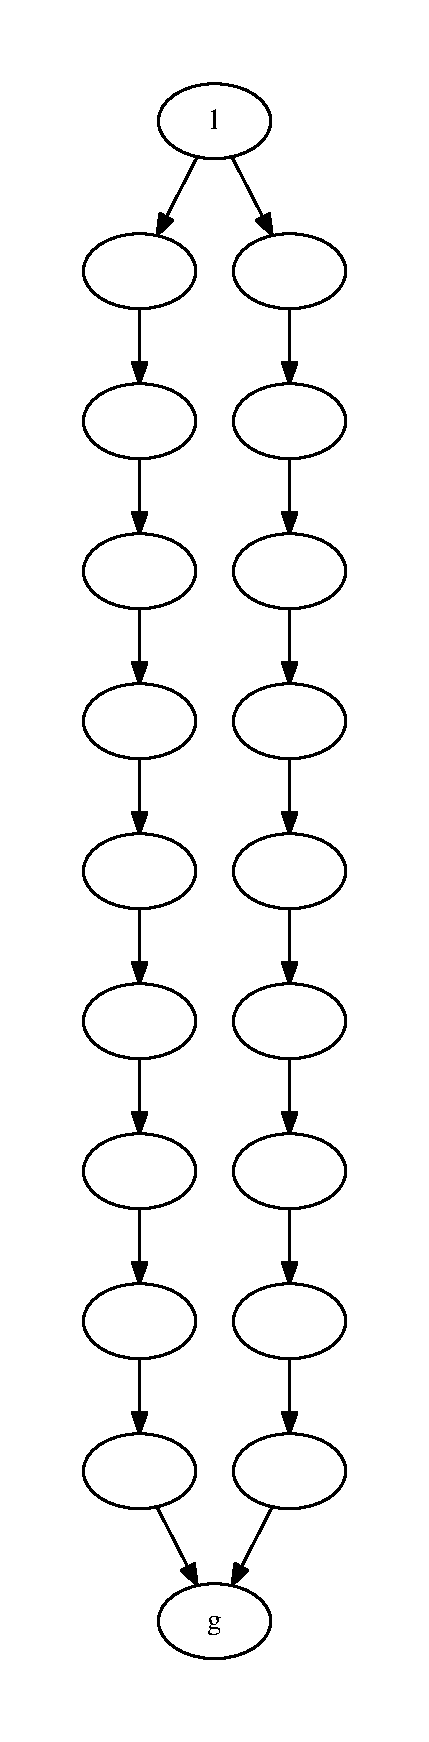
\includegraphics[height=.9\textheight]{figure/patterns/pattern1}
	\hfill
	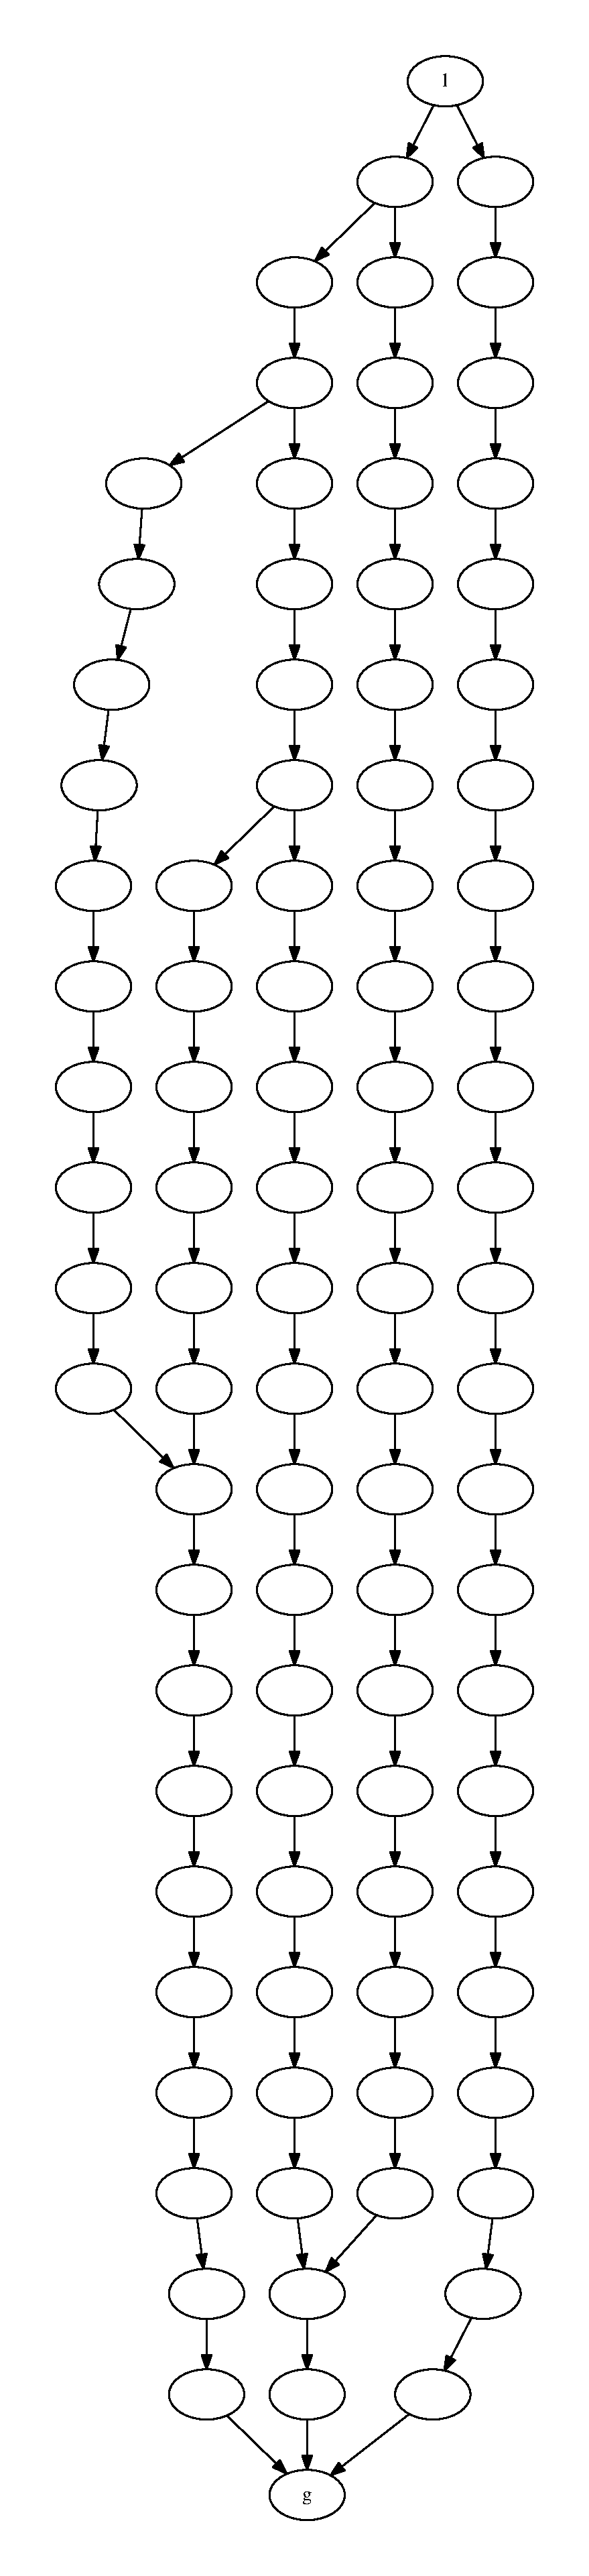
\includegraphics[height=.9\textheight]{figure/patterns/pattern2}
	\hfill
	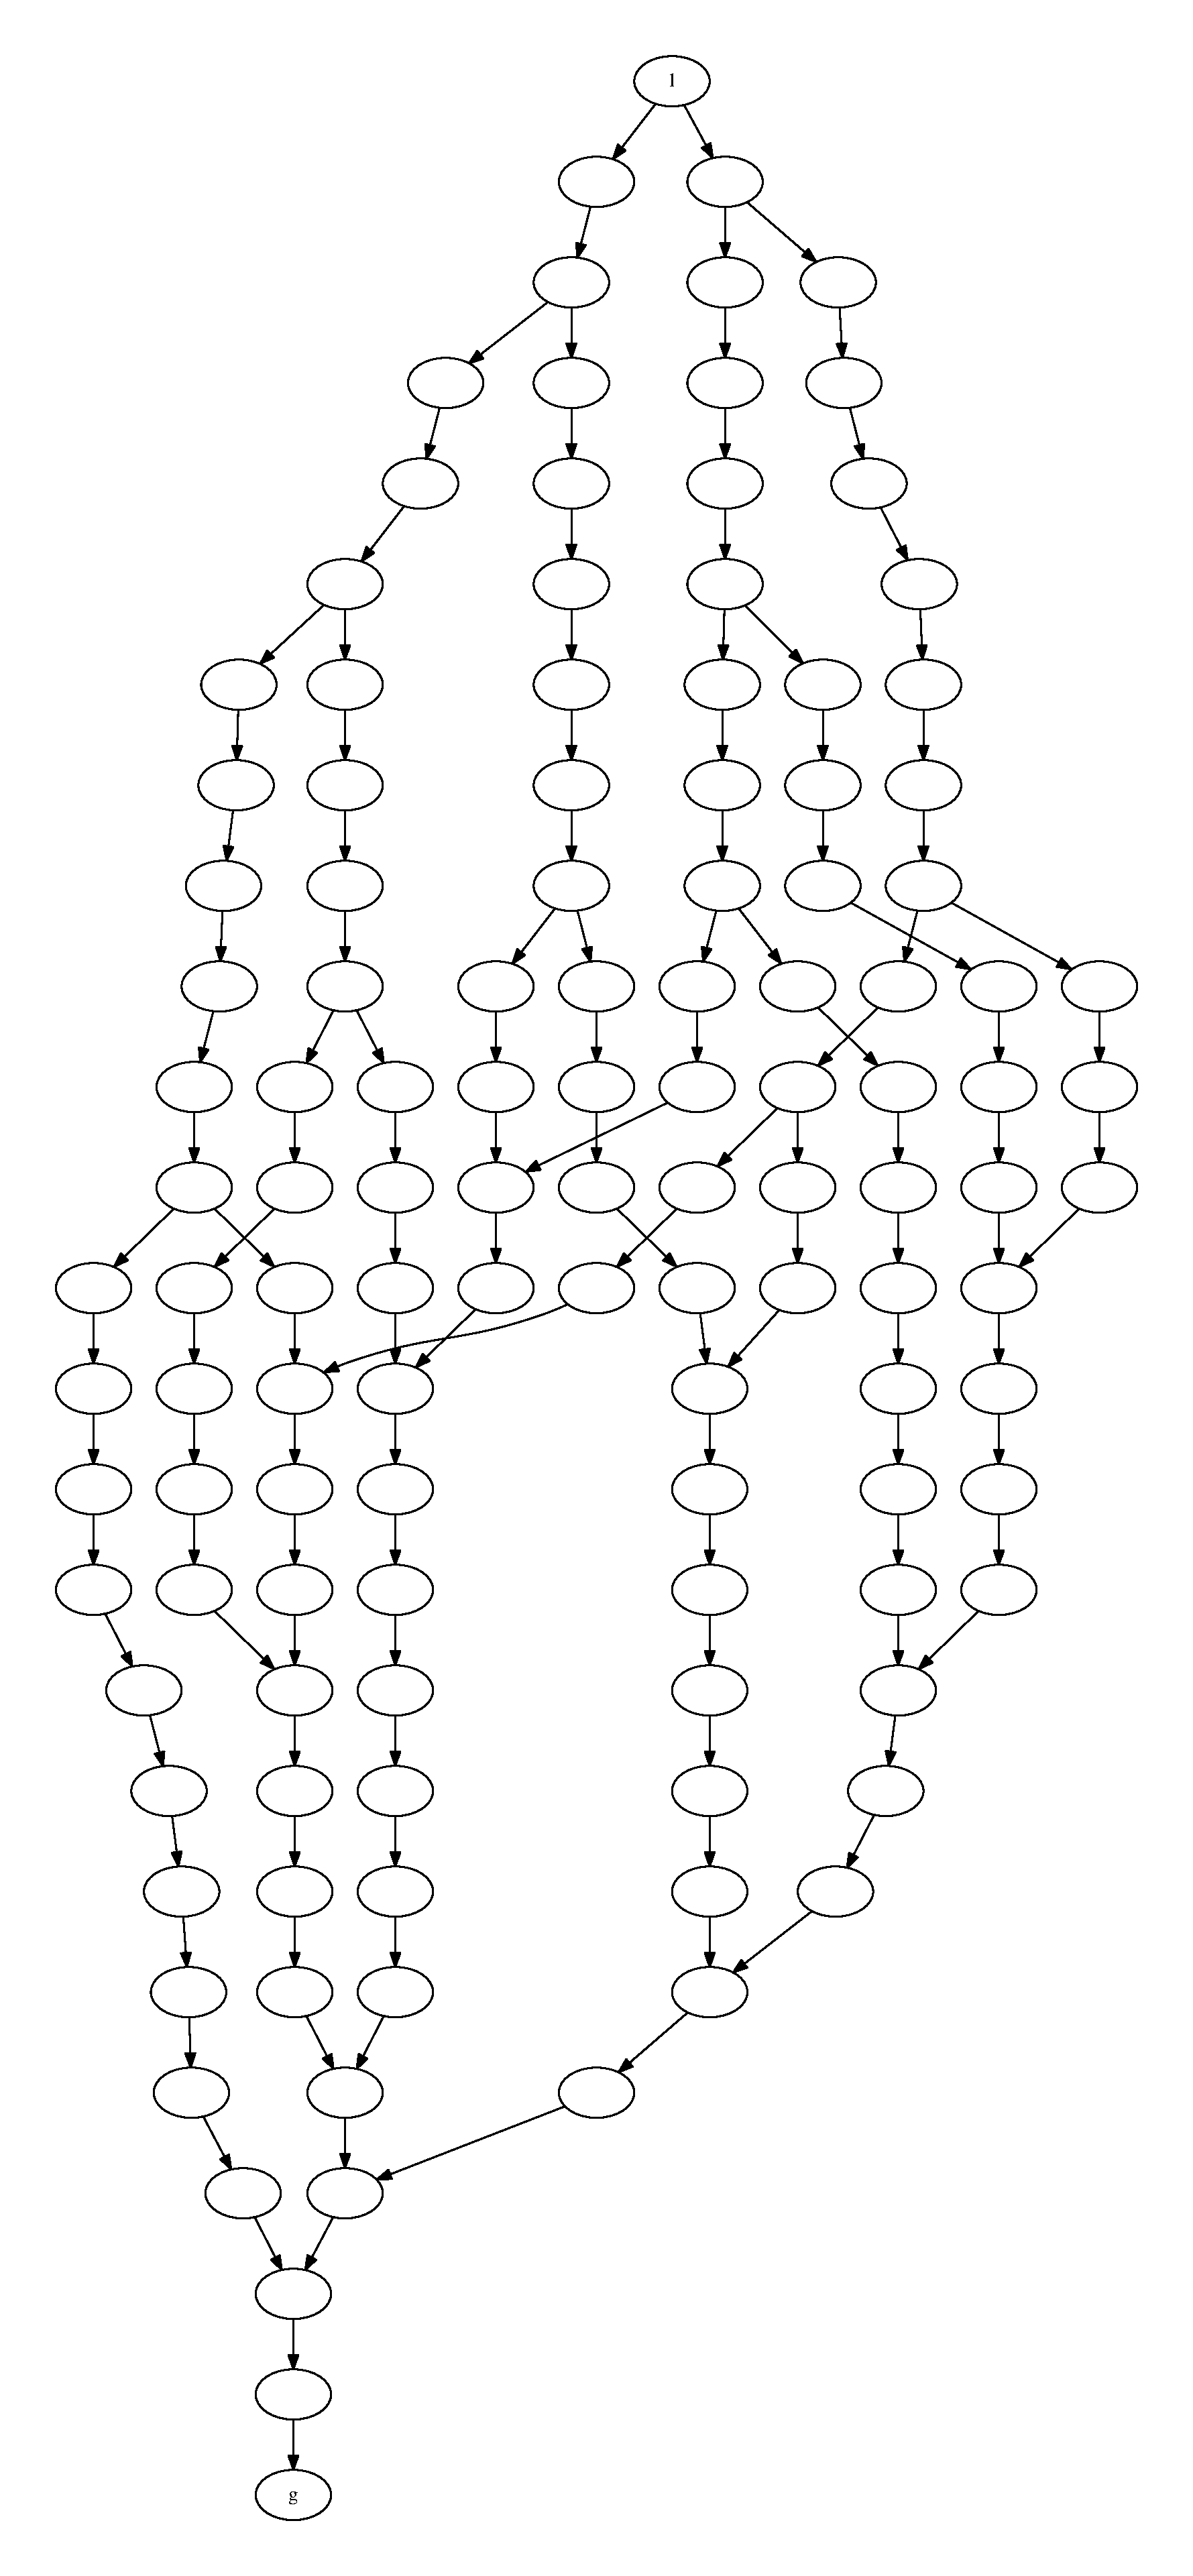
\includegraphics[height=.9\textheight]{figure/patterns/pattern3}
	\hfill
\end{figure}
\end{frame}
}

\section{Future}

\begin{frame}{What to try}

\begin{itemize}
\item
More meaningful experimental computational

\vspace{1em}

\item
Attempt to find some formal language which includes the geodesics of Fabrykowski-Gupta

\vspace{1em}

\item
Consider different groups of intermediate growth: Br\"onnimann's thesis\footcite{Julie2016GeodesicGrowth} was not exhaustive

\vspace{1em}

\item
Consider virtually nilpotent groups that are not known a priori to have only polynomial or exponential growth

\end{itemize}

\end{frame}

\begin{frame}{References}
\printbibliography[heading=none]
\end{frame}

\begin{frame}[standout]
Thanks!
\end{frame}

\end{document}